\documentclass[architecture]{compas2018}
%%%%%%%%%%%%%%%%%%%%%%%%%%%%%%%%%%%%%%%%%%%%%%%%%%%%%%%%%%%%%%%%%%%%%

\toappear{1} % Conserver cette ligne pour la version finale

\usepackage{tikz}
\tikzset{
  hwblock/.style={draw, rectangle, rounded corners=.3, very thick, fill=black!5, font=\sf, minimum height=5ex},
  hwbus/.style={very thick,>=stealth},
  hwwire/.style={thin, >=stealth, },
  hwword/.style={draw, rectangle, minimum height=3ex},
  bitwidth/.style={font=\scriptsize,midway,right}
}

\newcommand{\reg}{\textit{reg}}
\newcommand{\const}{\textit{const}}
\newcommand{\shiftval}{\textit{shiftval}}
\newcommand{\cond}{\textit{cond}}
\newcommand{\ctr}{\textit{ctr}}
\newcommand{\size}{\textit{size}}
\newcommand{\addr}{\textit{addr}}

\begin{document}

\title{Une architecture de von Neumann à bus bit-série}

\author{too many to mention}

\address{
  % \begin{tabular}{cc}
  %   ENS-Lyon & INSA Lyon \\
  %   \texttt{nom.prenom@ens-lyon.org} \\
  % \end{tabular}
}

\date{\today}

\maketitle

\begin{abstract}
La taille
  de ce résumé peut atteindre une dizaine de lignes.
  \MotsCles{un maximum de 5 mots significatifs, en français, doivent être 
    isolés sous forme de mots-clés.}
\end{abstract}


\section{Syntaxe de l'assembleur}

Les registres généralistes sont notés r0 à r7.
Ils sont tous parfaitement identiques, sauf r7 qui reçoit l'adresse de retour en cas de \texttt{call}.

Les instructions commencent toutes par un mnémonique, suivi des opérandes, le tout séparé par des espaces.

Les instructions ALU viennent en version 2 et 3 opérandes, la destination venant toujours en premier.
Par exemple, \\
 \begin{tabular}{lcl}
 \texttt{add2 r0 r1}&& réalise $r_0 \leftarrow r_0+r_1$. \\
 \texttt{add3 r0 r1 r2}&& réalise $r_0 \leftarrow r_1+r_2$.
 \end{tabular}
 
Le suffixe \texttt{i} signifie que le dernier opérande est une constante immédiate, par exemple:\\
 \begin{tabular}{lcl}
 \texttt{add2 r0 1}&& réalise $r_0 \leftarrow r_0+1$. \\
 \end{tabular}

L'assemblage commence à l'adresse 0, qui est celle à laquelle notre processeur démarre.

 
Sucre syntaxique offert par l'assembleur:
\begin{itemize}
\item On peut utiliser des labels pour les sauts.
\item Le mot-clé \texttt{.const n xxxx}  réserve $n$ bits de mémoire, initialisés à la constante xxxx, qui est priée de tenir sur $n$ bits.
\item Les constante hexadécimales sont préfixées par \texttt{0x}, par exemple \texttt{0xff}
\item Le commentaire est introduit par un point-virgule \texttt{;}
\end{itemize}
 

Exemple de programme :
\begin{verbatim}
  let r0 17     ; l'assembleur va calculer combien de bits il faut pour 17
boucle:	
  sub2i r0 1    ; encodé en 9 bits, et ceci est un commentaire
  jumpif nz boucle  ; encodé en 16 bits, signifie  jump -25 
\end{verbatim}

\section{Les instructions et leur encodage}



La table \ref{tab:opcodes} décrit l'opcode qui commence chaque instruction.

Remarques en vrac: 
\begin{itemize}
\item le not logique est implémenté par xor -1
\item la direction du shift est encodée dans un bit après l'instruction pour économiser un opcode. On aurait pu définir deux opcodes comme pour \texttt{uread}/\texttt{sread} mais c'est plus rigolo de lire \texttt{shift left r1 1}.
\end{itemize}


\begin{table}[!h]
  \caption{Liste des instructions.}
  \label{tab:opcodes}

  Les opérandes d'une instruction la suivent en mémoire. Ils sont encodés comme suit:
  \begin{itemize}
\item \textit{reg} $\in \{\mathtt{r0}, \mathtt{r1}, ..., \mathtt{r7}\}$ et est encodé par le numéro du registre en binaire.
\item \textit{const}, \textit{shiftval} et \textit{addr} sont définis par la table \ref{tab:constantes}. La dernière colonne de la table  \ref{tab:opcodes} précise si une constante est étendue avec son signe (s) ou des zéros (z).   
\item  \textit{cond} est défini par la table~\ref{tab:conditions}.
\item \ctr\ est défini par la table~\ref{tab:counters}.
\item \textit{dir} peut être le mnemnonique \texttt{left}, encodé par 0, ou le mnemonique \texttt{right}, encodé par 1.
\end{itemize}
\begin{center}
  \begin{tabular}{|l|l|l|l|l|c|}
    \hline  
    opcode  & mnemonic        & operands                      & description                                          & ext. & {MàJ flags} \\
    \hline  
    \hline  
    0000    & \texttt{add2}   & \reg\ \reg\                   & addition                                             &      & zcvn        \\
    \hline
    0001    & \texttt{add2i}  & \reg\ \const\                 & add immediate constant                               & z    & zcvn        \\
    \hline
    0010    & \texttt{sub2}   & \reg\ \reg\                   & subtraction                                          &      & zcvn        \\
    \hline
    0011    & \texttt{sub2i}  & \reg\ \const\                 & subtract immediate constant                          & z    & zcvn        \\
    \hline
    0100    & \texttt{cmp}    & \reg\ \reg\                   & comparison                                           &      & zcvn        \\
    \hline
    0101    & \texttt{cmpi}   & \reg\ \const\                 & comparison with immediate constant                   & s    & zcvn        \\
    \hline
    0110    & \texttt{let}    & \reg\ \reg\                   & register copy                                        &      &             \\
    \hline
    0111    & \texttt{leti}   & \reg\ \const\                 & fill register with constant                          & s    &             \\
    \hline
    1000    & \texttt{shift}  & \textit{dir} \reg\ \shiftval\ & logical shift                                        &      & zcn         \\
    \hline
    10010   & \texttt{readze} & \ctr\ \size\ \reg\            & read \size\ memory bits (zero-extended) to \reg\     &      &             \\
    10011   & \texttt{readse} & \ctr\ \size\ \reg\            & read \size\ memory bits (sign-extended) to \reg\     &      &             \\
    \hline
    1010    & \texttt{jump}   & \addr\                        & relative jump                                        &      &             \\
    \hline
    1011    & \texttt{jumpif} & \cond\ \addr\                 & conditional relative jump                            &      &             \\
    \hline
    110000  & \texttt{or2}    & \reg\ \reg\                   & logical bitwise or                                   &      & zcn         \\
    \hline
    110001  & \texttt{or2i}   & \reg\ \const\                 & logical bitwise or                                   & {z}  & zcn         \\
    \hline
    110010  & \texttt{and2}   & \reg\ \reg\                   & logical bitwise and                                  &      & zcn         \\
    \hline
    110011  & \texttt{and2i}  & \reg\ \const\                 & logical bitwise and                                  & {z}  & zcn         \\
    \hline
    110100  & \texttt{write}  & \ctr\ \size\ \reg\            & write the lower \size\ bits of \reg\ to mem          &      &             \\
    \hline
    110101  & \texttt{call}   & \addr\                        & sub-routine call                                     & s    &             \\
    \hline
    110110  & \texttt{setctr} & \ctr\ \reg\                   & set one of the four counters to the content of \reg\ &      &             \\
    \hline
    110111  & \texttt{getctr} & \ctr\ \reg\                   & copy the current value of a counter to \reg\         &      &             \\
    \hline
    1110000 & \texttt{push}   & \reg\                         & push value of register on stack                      &      &             \\
    \hline
    1110001 & \texttt{return} &                               & return from subroutine                               &      &             \\
    \hline
    1110010 & \texttt{add3}   & \reg\ \reg\ \reg\             &                                                      &      & zcvn        \\
    \hline
    1110011 & \texttt{add3i}  & \reg\ \reg\ \const\           &                                                      & z    & zcvn        \\
    \hline
    1110100 & \texttt{sub3}   & \reg\ \reg\ \reg\             &                                                      &      & zcvn        \\
    \hline
    1110101 & \texttt{sub3i}  & \reg\ \reg\ \const\           &                                                      & z    & zcvn        \\
    \hline
    1110110 & \texttt{and3}   & \reg\  \reg\ \reg\            &                                                      &      & zcn         \\
    \hline
    1110111 & \texttt{and3i}  & \reg\ \reg\ \const\           &                                                      & {z}  & zcn         \\
    \hline
    1111000 & \texttt{or3}    & \reg\ \reg\ \reg\             &                                                      &      & zcn         \\
    \hline
    1111001 & \texttt{or3i}   & \reg\ \reg\ \const\           &                                                      & {z}  & zcn         \\
    \hline
    1111010 & \texttt{xor3}   & \reg\ \reg\ \reg\             &                                                      &      & zcn         \\
    \hline
    1111011 & \texttt{xor3i}  & \reg\ \reg\ \const\           &                                                      & {z}  & zcn         \\
    \hline
    1111100 & \texttt{asr3}   & \reg\  \reg\ \shiftval\       &                                                      &      & zcn         \\
    \hline
    1111101 & \texttt{}       &                               & reserved                                             &      &             \\
    \hline
    1111110 & \texttt{}       &                               & reserved                                             &      &             \\
    \hline
    1111111 & \texttt{}       &                               & reserved                                             &      &             \\
    \hline
  \end{tabular}
\end{center}
\end{table}


\begin{table}
  \label{tab:constantes}
  \centering
  \caption{Encodage des constantes}
  \begin{tabular}{|l|l|}
    \hline
    \multicolumn{2}{|c|}{\textit{addr} : Encodage \emph{prefix-free} des adresses et déplacements} \\
    \hline
    0 + 8 bits    & adresse ou déplacement sur 8 bits                                              \\
    \hline
    10 + 16 bits  &                                                                                \\
    \hline
    110 + 32 bits &                                                                                \\
    \hline
    111 + 64 bits &                                                                                \\
    \hline
    \hline
    \multicolumn{2}{|c|}{\textit{shiftval} : Encodage \emph{prefix-free} des constantes de shift}  \\
    \hline
    0 + 6 bits    & constante entre 0 et 63                                                        \\
    \hline
    1             & constante 1                                                                    \\
    \hline
    \hline
    \multicolumn{2}{|c|}{\textit{const} : Encodage \emph{prefix-free} des constantes ALU}          \\
    \hline
    0 + 1 bit     & constante 0 ou 1                                                               \\
    \hline
    10 + 8 bits   & octet                                                                          \\
    \hline
    110 + 32 bits &                                                                                \\
    \hline
    111 + 64 bits &                                                                                \\
    \hline
    \hline
    \multicolumn{2}{|c|}{\textit{size} : Encodage \emph{prefix-free} des tailles mémoire}          \\
    \hline
    00            & 1 bit                                                                          \\
    \hline
    01            & 4 bits                                                                         \\
    \hline
    100           & 8 bits                                                                         \\
    \hline
    101           & 16 bits                                                                        \\
    \hline
    110           & 32 bits                                                                        \\
    \hline
    111           & 64 bits                                                                        \\
    \hline
  \end{tabular}
\end{table}



\subsection{Les instructions de branchement }
\label{sec:jumpcallret}

Soit $a$ l'adresse du premier bit suivant l'instruction \texttt{jump} ou \texttt{call} (i.e. la valeur du PC lorsqu'il a fini de lire l'instruction et ses opérandes).
Soit $d$ la valeur de déplacement (encodée dans une constante de type \textit{addr}, et signée).

L'instruction \texttt{jump} réalise $\mathtt{pc}\leftarrow a + c$.
L'instruction \texttt{jumpif} aussi, mais seulement si la condition est vraie.

La condition  est encodée sur trois bits  selon la table~\ref{tab:conditions}.
\newcommand{\bool}{\mathbb{B}}
\newcommand{\booland}{\wedge}
\newcommand{\boolor}{\vee}
\newcommand{\boolnot}[1]{\overline{#1}}
\begin{table} 
  \caption{Condition codes}
  \label{tab:conditions}
\begin{center}
  \begin{tabular}{|c|c|c||l||l|c|}
    \hline  
      &   &   & mnemonic                  & description (after \texttt{cmp} op1 op2)           & {implem.}                                                                           \\
    \hline  
    \hline  
    0 & 0 & 0 & \texttt{eq}, \texttt{z}   & equal, op1 $=$ op2                                 & $z$                                                                                 \\
    \hline
    0 & 0 & 1 & \texttt{neq}, \texttt{nz} & not equal, op1 $\neq$ op2                          & $\boolnot{z}$                                                                       \\
    \hline
    0 & 1 & 0 & \texttt{sgt}              & signed greater than, op1 $>$ op2, two's complement & $\boolnot{z} \booland (n \booland {v}) \boolor (\boolnot{n} \booland \boolnot{v}) $ \\
    \hline
    0 & 1 & 1 & \texttt{slt}              & signed smaller than, op1 $<$ op2, two's complement & $(n \booland \boolnot{v}) \boolor (\boolnot{n} \booland v) $                        \\
    \hline
    1 & 0 & 0 & \texttt{gt}               & op1 $>$ op2, unsigned                              & $\boolnot{z} \booland \boolnot{c}$                                                  \\
    \hline
    1 & 0 & 1 & \texttt{ge}, \texttt{nc}  & op1 $\ge$ op2, unsigned                            & $\boolnot{c}$                                                                       \\
    \hline
    1 & 1 & 0 & \texttt{lt}, \texttt{c}   & op1 $<$ op2, unsigned                              & $c$                                                                                 \\
    \hline
    1 & 1 & 1 & {\texttt{v}}              & {two's complement overflow}                        & {$v$}                                                                               \\
    \hline
  \end{tabular}
\end{center}
\end{table} 

La différence entre \texttt{sgt} et \texttt{gt} s'observe par exemple sur la comparaison entre \texttt{r0} et -1.

L'instruction \texttt{call} copie $\texttt{a}$ dans $r_{7}$, puis réalise $\mathtt{pc} \leftarrow \texttt{d}$
(c'est un peu bizarre de sauter à des adresses négatives mais du coup \emph{addr} est toujours signé).

L'instruction \texttt{return} copie \texttt{r7} dans \texttt{pc}.

\subsection{Les instructions d'accès mémoire}
\label{sec:mem}

\begin{figure}[h]
  \caption{Overview of the processor-memory interface}
  \label{fig:overview}
    \begin{center}
  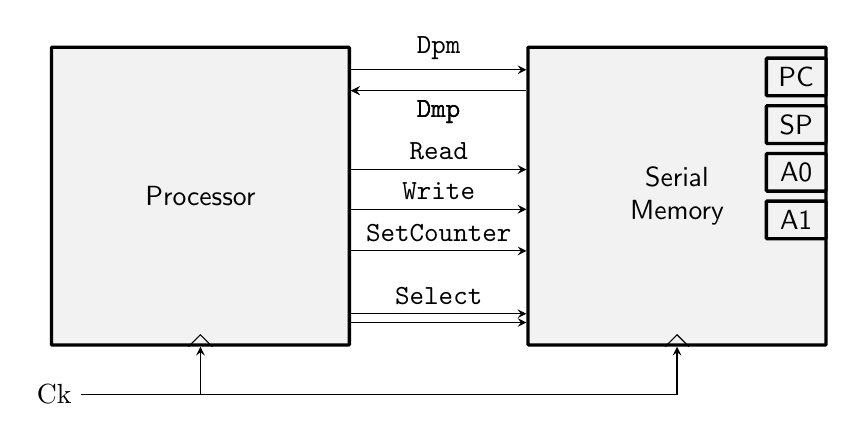
\begin{tikzpicture}
    \node[hwblock, minimum width=25ex,minimum height=25ex] (p) at (-10ex,0)  {Processor} ;
    \node[hwblock, minimum width=25ex,minimum height=25ex, align=center] (m) at (30ex,0)  {Serial\\ Memory} ;
    \node[hwblock,minimum height=3ex,minimum width=5ex] (pc) at (40ex,10ex)  {PC} ;
    \node[hwblock,minimum height=3ex,minimum width=5ex] (pc) at (40ex,6ex)  {SP} ;
    \node[hwblock,minimum height=3ex,minimum width=5ex] (pc) at (40ex,2ex)  {A0} ;
    \node[hwblock,minimum height=3ex,minimum width=5ex] (pc) at (40ex,-2ex)  {A1} ;
    \draw[hwwire,->] (p.40) -- (m.140) node[midway,above]{\texttt{Dpm}};
    \draw[hwwire,<-] (p.35) -- (m.145) node[midway,below]{\texttt{Dmp}};

    \draw[hwwire,->] (p.10) -- (m.170) node[midway,above]{\texttt{Read}};
    \draw[hwwire,->] (p.355) -- (m.185) node[midway,above]{\texttt{Write}};
    \draw[hwwire,->] (p.340) -- (m.200) node[midway,above]{\texttt{SetCounter}};
    \draw[hwwire,->] (p.322) -- (m.218) node[midway,above]{\texttt{Select}};
    \draw[hwwire,->] (p.320) -- (m.220) node[midway,above]{};
    \draw[hwwire,<-] (p.35) -- (m.145) node[midway,below]{\texttt{Dmp}};
    \draw[hwwire,<-] (m.south) -- ++(0,-4ex) -- ++(-50ex,0) node[left]{Ck};
    \draw[hwwire,<-] (p.south) -- ++(0,-4ex);
    \draw[hwwire,-] (p.south)  ++(-1ex, 0) -- ++(1ex,1ex) -- ++(1ex,-1ex); % horloge
    \draw[hwwire,-] (m.south)  ++(-1ex, 0) -- ++(1ex,1ex) -- ++(1ex,-1ex); % horloge
  \end{tikzpicture}
  \end{center}
\end{figure}


On a 4 compteurs d'adresses, chacun  répliqué dans le processeur et dans la mémoire (Table~\ref{tab:counters}).


Les instructions \texttt{readze}, \texttt{readse} et \texttt{write} lisent ou écrivent le nombre spécifié de bits tout en incrémentant les compteurs correspondant.

On peut émuler une instruction de lecture/écriture mémoire d'un processeur classique en deux instructions: un \texttt{setctr} puis un \texttt{readze} ou \texttt{readse} ou \texttt{write}.

Les instructions \texttt{push} et \texttt{pop} implémentent une pile descendante en mémoire: 
\begin{itemize}
\item \texttt{push} \emph{size} \emph{reg} réalise: \\
  $\mathit{sp}\leftarrow \mathit{sp}-\mathit{size}$\\ \texttt{setctr} \textit{sp}\\ \texttt{write}  \textit{sp} \textit{size} \textit{reg} \\   $\mathit{sp}\leftarrow \mathit{sp}-\mathit{size}$\\ \texttt{setctr} \textit{sp}
\item \texttt{pop} \emph{size} \emph{reg} est un raccourci offert par l'assembleur pour \\\texttt{readze} \textit{sp} \emph{size} \emph{reg}\\
  
\end{itemize}

\begin{table} 
  \caption{Counters. Ces deux bits sont transmis sur le signal \texttt{Select} de la figure~\ref{fig:overview}. }
  \label{tab:counters}
\begin{center}
  \begin{tabular}{|l|l|l|}
    \hline  
  encoding  & mnemonic & description \\
    \hline  
    \hline  
    00& \texttt{pc} &  program counter\\
    \hline
    01& \texttt{sp} & stack pointer\\
    \hline
    10& \texttt{a0} &  generic address counter\\
    \hline
    11& \texttt{a1} &  generic address counter\\
    \hline
  \end{tabular}
\end{center}
\end{table}




\end{document}








